% Options for packages loaded elsewhere
\PassOptionsToPackage{unicode}{hyperref}
\PassOptionsToPackage{hyphens}{url}
\PassOptionsToPackage{dvipsnames,svgnames,x11names}{xcolor}
%
\documentclass[
  letterpaper,
  DIV=11,
  numbers=noendperiod]{scrartcl}

\usepackage{amsmath,amssymb}
\usepackage{iftex}
\ifPDFTeX
  \usepackage[T1]{fontenc}
  \usepackage[utf8]{inputenc}
  \usepackage{textcomp} % provide euro and other symbols
\else % if luatex or xetex
  \usepackage{unicode-math}
  \defaultfontfeatures{Scale=MatchLowercase}
  \defaultfontfeatures[\rmfamily]{Ligatures=TeX,Scale=1}
\fi
\usepackage{lmodern}
\ifPDFTeX\else  
    % xetex/luatex font selection
\fi
% Use upquote if available, for straight quotes in verbatim environments
\IfFileExists{upquote.sty}{\usepackage{upquote}}{}
\IfFileExists{microtype.sty}{% use microtype if available
  \usepackage[]{microtype}
  \UseMicrotypeSet[protrusion]{basicmath} % disable protrusion for tt fonts
}{}
\makeatletter
\@ifundefined{KOMAClassName}{% if non-KOMA class
  \IfFileExists{parskip.sty}{%
    \usepackage{parskip}
  }{% else
    \setlength{\parindent}{0pt}
    \setlength{\parskip}{6pt plus 2pt minus 1pt}}
}{% if KOMA class
  \KOMAoptions{parskip=half}}
\makeatother
\usepackage{xcolor}
\setlength{\emergencystretch}{3em} % prevent overfull lines
\setcounter{secnumdepth}{-\maxdimen} % remove section numbering
% Make \paragraph and \subparagraph free-standing
\makeatletter
\ifx\paragraph\undefined\else
  \let\oldparagraph\paragraph
  \renewcommand{\paragraph}{
    \@ifstar
      \xxxParagraphStar
      \xxxParagraphNoStar
  }
  \newcommand{\xxxParagraphStar}[1]{\oldparagraph*{#1}\mbox{}}
  \newcommand{\xxxParagraphNoStar}[1]{\oldparagraph{#1}\mbox{}}
\fi
\ifx\subparagraph\undefined\else
  \let\oldsubparagraph\subparagraph
  \renewcommand{\subparagraph}{
    \@ifstar
      \xxxSubParagraphStar
      \xxxSubParagraphNoStar
  }
  \newcommand{\xxxSubParagraphStar}[1]{\oldsubparagraph*{#1}\mbox{}}
  \newcommand{\xxxSubParagraphNoStar}[1]{\oldsubparagraph{#1}\mbox{}}
\fi
\makeatother

\usepackage{color}
\usepackage{fancyvrb}
\newcommand{\VerbBar}{|}
\newcommand{\VERB}{\Verb[commandchars=\\\{\}]}
\DefineVerbatimEnvironment{Highlighting}{Verbatim}{commandchars=\\\{\}}
% Add ',fontsize=\small' for more characters per line
\usepackage{framed}
\definecolor{shadecolor}{RGB}{241,243,245}
\newenvironment{Shaded}{\begin{snugshade}}{\end{snugshade}}
\newcommand{\AlertTok}[1]{\textcolor[rgb]{0.68,0.00,0.00}{#1}}
\newcommand{\AnnotationTok}[1]{\textcolor[rgb]{0.37,0.37,0.37}{#1}}
\newcommand{\AttributeTok}[1]{\textcolor[rgb]{0.40,0.45,0.13}{#1}}
\newcommand{\BaseNTok}[1]{\textcolor[rgb]{0.68,0.00,0.00}{#1}}
\newcommand{\BuiltInTok}[1]{\textcolor[rgb]{0.00,0.23,0.31}{#1}}
\newcommand{\CharTok}[1]{\textcolor[rgb]{0.13,0.47,0.30}{#1}}
\newcommand{\CommentTok}[1]{\textcolor[rgb]{0.37,0.37,0.37}{#1}}
\newcommand{\CommentVarTok}[1]{\textcolor[rgb]{0.37,0.37,0.37}{\textit{#1}}}
\newcommand{\ConstantTok}[1]{\textcolor[rgb]{0.56,0.35,0.01}{#1}}
\newcommand{\ControlFlowTok}[1]{\textcolor[rgb]{0.00,0.23,0.31}{\textbf{#1}}}
\newcommand{\DataTypeTok}[1]{\textcolor[rgb]{0.68,0.00,0.00}{#1}}
\newcommand{\DecValTok}[1]{\textcolor[rgb]{0.68,0.00,0.00}{#1}}
\newcommand{\DocumentationTok}[1]{\textcolor[rgb]{0.37,0.37,0.37}{\textit{#1}}}
\newcommand{\ErrorTok}[1]{\textcolor[rgb]{0.68,0.00,0.00}{#1}}
\newcommand{\ExtensionTok}[1]{\textcolor[rgb]{0.00,0.23,0.31}{#1}}
\newcommand{\FloatTok}[1]{\textcolor[rgb]{0.68,0.00,0.00}{#1}}
\newcommand{\FunctionTok}[1]{\textcolor[rgb]{0.28,0.35,0.67}{#1}}
\newcommand{\ImportTok}[1]{\textcolor[rgb]{0.00,0.46,0.62}{#1}}
\newcommand{\InformationTok}[1]{\textcolor[rgb]{0.37,0.37,0.37}{#1}}
\newcommand{\KeywordTok}[1]{\textcolor[rgb]{0.00,0.23,0.31}{\textbf{#1}}}
\newcommand{\NormalTok}[1]{\textcolor[rgb]{0.00,0.23,0.31}{#1}}
\newcommand{\OperatorTok}[1]{\textcolor[rgb]{0.37,0.37,0.37}{#1}}
\newcommand{\OtherTok}[1]{\textcolor[rgb]{0.00,0.23,0.31}{#1}}
\newcommand{\PreprocessorTok}[1]{\textcolor[rgb]{0.68,0.00,0.00}{#1}}
\newcommand{\RegionMarkerTok}[1]{\textcolor[rgb]{0.00,0.23,0.31}{#1}}
\newcommand{\SpecialCharTok}[1]{\textcolor[rgb]{0.37,0.37,0.37}{#1}}
\newcommand{\SpecialStringTok}[1]{\textcolor[rgb]{0.13,0.47,0.30}{#1}}
\newcommand{\StringTok}[1]{\textcolor[rgb]{0.13,0.47,0.30}{#1}}
\newcommand{\VariableTok}[1]{\textcolor[rgb]{0.07,0.07,0.07}{#1}}
\newcommand{\VerbatimStringTok}[1]{\textcolor[rgb]{0.13,0.47,0.30}{#1}}
\newcommand{\WarningTok}[1]{\textcolor[rgb]{0.37,0.37,0.37}{\textit{#1}}}

\providecommand{\tightlist}{%
  \setlength{\itemsep}{0pt}\setlength{\parskip}{0pt}}\usepackage{longtable,booktabs,array}
\usepackage{calc} % for calculating minipage widths
% Correct order of tables after \paragraph or \subparagraph
\usepackage{etoolbox}
\makeatletter
\patchcmd\longtable{\par}{\if@noskipsec\mbox{}\fi\par}{}{}
\makeatother
% Allow footnotes in longtable head/foot
\IfFileExists{footnotehyper.sty}{\usepackage{footnotehyper}}{\usepackage{footnote}}
\makesavenoteenv{longtable}
\usepackage{graphicx}
\makeatletter
\def\maxwidth{\ifdim\Gin@nat@width>\linewidth\linewidth\else\Gin@nat@width\fi}
\def\maxheight{\ifdim\Gin@nat@height>\textheight\textheight\else\Gin@nat@height\fi}
\makeatother
% Scale images if necessary, so that they will not overflow the page
% margins by default, and it is still possible to overwrite the defaults
% using explicit options in \includegraphics[width, height, ...]{}
\setkeys{Gin}{width=\maxwidth,height=\maxheight,keepaspectratio}
% Set default figure placement to htbp
\makeatletter
\def\fps@figure{htbp}
\makeatother

\KOMAoption{captions}{tableheading}
\makeatletter
\@ifpackageloaded{caption}{}{\usepackage{caption}}
\AtBeginDocument{%
\ifdefined\contentsname
  \renewcommand*\contentsname{Table of contents}
\else
  \newcommand\contentsname{Table of contents}
\fi
\ifdefined\listfigurename
  \renewcommand*\listfigurename{List of Figures}
\else
  \newcommand\listfigurename{List of Figures}
\fi
\ifdefined\listtablename
  \renewcommand*\listtablename{List of Tables}
\else
  \newcommand\listtablename{List of Tables}
\fi
\ifdefined\figurename
  \renewcommand*\figurename{Figure}
\else
  \newcommand\figurename{Figure}
\fi
\ifdefined\tablename
  \renewcommand*\tablename{Table}
\else
  \newcommand\tablename{Table}
\fi
}
\@ifpackageloaded{float}{}{\usepackage{float}}
\floatstyle{ruled}
\@ifundefined{c@chapter}{\newfloat{codelisting}{h}{lop}}{\newfloat{codelisting}{h}{lop}[chapter]}
\floatname{codelisting}{Listing}
\newcommand*\listoflistings{\listof{codelisting}{List of Listings}}
\makeatother
\makeatletter
\makeatother
\makeatletter
\@ifpackageloaded{caption}{}{\usepackage{caption}}
\@ifpackageloaded{subcaption}{}{\usepackage{subcaption}}
\makeatother

\ifLuaTeX
  \usepackage{selnolig}  % disable illegal ligatures
\fi
\usepackage{bookmark}

\IfFileExists{xurl.sty}{\usepackage{xurl}}{} % add URL line breaks if available
\urlstyle{same} % disable monospaced font for URLs
\hypersetup{
  pdftitle={Mini Project 1},
  pdfauthor={Gwynnie Hayes},
  colorlinks=true,
  linkcolor={blue},
  filecolor={Maroon},
  citecolor={Blue},
  urlcolor={Blue},
  pdfcreator={LaTeX via pandoc}}


\title{Mini Project 1}
\author{Gwynnie Hayes}
\date{}

\begin{document}
\maketitle


\subsection{Importing Data}\label{importing-data}

\begin{Shaded}
\begin{Highlighting}[]
\FunctionTok{library}\NormalTok{(tidyverse)}
\FunctionTok{library}\NormalTok{(dplyr)}
\FunctionTok{library}\NormalTok{(sf)}
\FunctionTok{library}\NormalTok{(tmap)}
\FunctionTok{library}\NormalTok{(maps)}
\FunctionTok{library}\NormalTok{(viridis)}
\FunctionTok{library}\NormalTok{(htmltools)}
\FunctionTok{library}\NormalTok{(glue)}
\FunctionTok{library}\NormalTok{(leaflet)}

\NormalTok{us\_states }\OtherTok{\textless{}{-}} \FunctionTok{map\_data}\NormalTok{(}\StringTok{"state"}\NormalTok{)}

\NormalTok{frogs }\OtherTok{\textless{}{-}} \FunctionTok{read.csv}\NormalTok{(}\StringTok{"\textasciitilde{}/Desktop/15/SDS264/data/most\_common\_frog.csv"}\NormalTok{) }\SpecialCharTok{|\textgreater{}}
  \FunctionTok{na.omit}\NormalTok{()}

\NormalTok{forests }\OtherTok{\textless{}{-}} \FunctionTok{read.csv}\NormalTok{(}\StringTok{"\textasciitilde{}/Desktop/15/SDS264/data/forests.csv"}\NormalTok{) }\SpecialCharTok{|\textgreater{}}
  \FunctionTok{mutate}\NormalTok{(}\StringTok{\textquotesingle{}forest\_cover\textquotesingle{}} \OtherTok{=}\NormalTok{ forest\_area}\SpecialCharTok{/}\NormalTok{land\_area }\SpecialCharTok{*} \DecValTok{100}\NormalTok{)}

\NormalTok{states }\OtherTok{\textless{}{-}} \FunctionTok{read\_sf}\NormalTok{(}\StringTok{"https://rstudio.github.io/leaflet/json/us{-}states.geojson"}\NormalTok{)}
\end{Highlighting}
\end{Shaded}

\subsection{Data Source}\label{data-source}

\section{Forest}\label{forest}

For my numerical maps, I looked at the percentage of land covered in
forest in the united states. I found this data in the USDA Forest
Service FIA Annual Report, this report is a pdf where I extracted the
values that I would need for this data set.

\section{Frogs}\label{frogs}

I wanted to look frogs for my categorical data. I found observations of
frogs on the website, inaturalist where you can export observations
based on specific criteria. I wanted to look at something more
interesting then just the most common frog in each state so i looked at
the most commonly observed frog that is deemed threatened.

\subsection{Joining with Polygons}\label{joining-with-polygons}

\begin{Shaded}
\begin{Highlighting}[]
\NormalTok{forests\_static }\OtherTok{\textless{}{-}}\NormalTok{ forests }\SpecialCharTok{|\textgreater{}}
  \FunctionTok{mutate}\NormalTok{(}\AttributeTok{state =} \FunctionTok{str\_to\_lower}\NormalTok{(state)) }\SpecialCharTok{|\textgreater{}}
  \FunctionTok{right\_join}\NormalTok{(us\_states, }\AttributeTok{by =} \FunctionTok{c}\NormalTok{(}\StringTok{"state"} \OtherTok{=} \StringTok{"region"}\NormalTok{)) }
\end{Highlighting}
\end{Shaded}

\begin{Shaded}
\begin{Highlighting}[]
\NormalTok{frogs\_static }\OtherTok{\textless{}{-}}\NormalTok{ frogs }\SpecialCharTok{|\textgreater{}}
  \FunctionTok{mutate}\NormalTok{(}\AttributeTok{state =} \FunctionTok{str\_to\_lower}\NormalTok{(state)) }\SpecialCharTok{|\textgreater{}}
  \FunctionTok{right\_join}\NormalTok{(us\_states, }\AttributeTok{by =} \FunctionTok{c}\NormalTok{(}\StringTok{"state"} \OtherTok{=} \StringTok{"region"}\NormalTok{))}
\end{Highlighting}
\end{Shaded}

\subsection{Static Maps}\label{static-maps}

\begin{Shaded}
\begin{Highlighting}[]
\NormalTok{forests\_static }\SpecialCharTok{|\textgreater{}}
  \FunctionTok{ggplot}\NormalTok{(}\AttributeTok{mapping =} \FunctionTok{aes}\NormalTok{(}\AttributeTok{x =}\NormalTok{ long, }\AttributeTok{y =}\NormalTok{ lat, }\AttributeTok{group =}\NormalTok{ group)) }\SpecialCharTok{+} 
  \FunctionTok{geom\_polygon}\NormalTok{(}\FunctionTok{aes}\NormalTok{(}\AttributeTok{fill =}\NormalTok{ forest\_cover), }\AttributeTok{color =} \StringTok{"black"}\NormalTok{, }\AttributeTok{linewidth =} \FloatTok{0.2}\NormalTok{) }\SpecialCharTok{+} 
  \FunctionTok{labs}\NormalTok{(}\AttributeTok{fill =} \StringTok{"\% Forest Coverage"}\NormalTok{, }\AttributeTok{title =} \StringTok{"Percent of Forest Coverage in each US State"}\NormalTok{, }\AttributeTok{x =} \StringTok{"Longitude"}\NormalTok{, }\AttributeTok{y =} \StringTok{"Latitude"}\NormalTok{, }\AttributeTok{caption =} \StringTok{"Data Source: USDA Forest Service FIA Annual Report"}\NormalTok{) }\SpecialCharTok{+}
  \FunctionTok{coord\_map}\NormalTok{() }\SpecialCharTok{+}
  \FunctionTok{scale\_fill\_viridis}\NormalTok{(}\AttributeTok{option =} \StringTok{"viridis"}\NormalTok{, }\AttributeTok{direction =} \SpecialCharTok{{-}}\DecValTok{1}\NormalTok{) }\SpecialCharTok{+}
  \FunctionTok{theme\_linedraw}\NormalTok{()}
\end{Highlighting}
\end{Shaded}

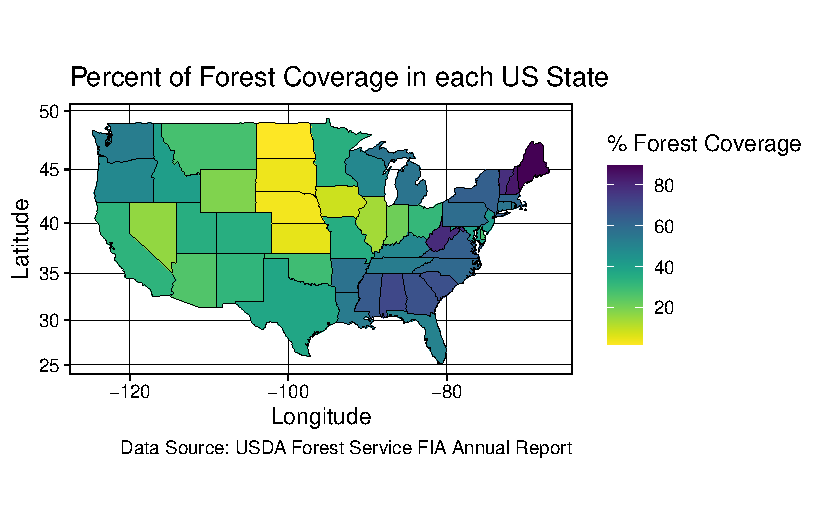
\includegraphics{MiniProject1_files/figure-pdf/unnamed-chunk-4-1.pdf}

alt text: This is a choropleth map of the United States that is looking
a the percentage of land area that is covered by forest in each state.
The x-axis is the longitude values of the United States which contain
values -120 - -80. The y-axis the latitude values of the United States
which contain values 25-50. This map is colored by the percentage forest
covereage with the most coverage being a dark purple while the least
coverage is a bright yellow. From this map we can see that states in the
East have a higher percentage of forest coverage while states in the
middle have a much lower percent forest coverage, then the west coast
has a medium amount of forest coverage.

\begin{Shaded}
\begin{Highlighting}[]
\NormalTok{frogs\_static }\SpecialCharTok{|\textgreater{}}
  \FunctionTok{ggplot}\NormalTok{(}\AttributeTok{mapping =} \FunctionTok{aes}\NormalTok{(}\AttributeTok{x =}\NormalTok{ long, }\AttributeTok{y =}\NormalTok{ lat, }\AttributeTok{group =}\NormalTok{ group)) }\SpecialCharTok{+} 
  \FunctionTok{geom\_polygon}\NormalTok{(}\FunctionTok{aes}\NormalTok{(}\AttributeTok{fill =}\NormalTok{ frog), }\AttributeTok{color =} \StringTok{"black"}\NormalTok{, }\AttributeTok{linewidth =} \FloatTok{0.2}\NormalTok{) }\SpecialCharTok{+} 
  \FunctionTok{labs}\NormalTok{(}\AttributeTok{fill =} \StringTok{"Frog Common Name"}\NormalTok{, }\AttributeTok{title =} \StringTok{"Most Observed Threatened Frog in Each State"}\NormalTok{, }\AttributeTok{x =} \StringTok{"Longitude"}\NormalTok{, }\AttributeTok{y =} \StringTok{"Latitude"}\NormalTok{, }\AttributeTok{caption =} \StringTok{"Data Source: https://www.inaturalist.org/observations?place\_id=1\&subview=map\&taxon\_id=25473\&threatened"}\NormalTok{) }\SpecialCharTok{+}
  \FunctionTok{scale\_fill\_manual}\NormalTok{(}\AttributeTok{values =} \FunctionTok{c}\NormalTok{(}\StringTok{"\#800000"}\NormalTok{, }
                               \StringTok{"\#9A6324"}\NormalTok{, }
                               \StringTok{"\#808000"}\NormalTok{, }
                               \StringTok{"\#469990"}\NormalTok{, }
                               \StringTok{"\#000075"}\NormalTok{, }
                               \StringTok{"\#000000"}\NormalTok{, }
                               \StringTok{"\#e6194B"}\NormalTok{, }
                               \StringTok{"\#f58231"}\NormalTok{, }
                               \StringTok{"\#ffe119"}\NormalTok{, }
                               \StringTok{"\#bfef45"}\NormalTok{, }
                               \StringTok{"\#3cb44b"}\NormalTok{, }
                               \StringTok{"\#42d4f4"}\NormalTok{, }
                               \StringTok{"\#4363d8"}\NormalTok{,}
                               \StringTok{"\#911eb4"}\NormalTok{, }
                               \StringTok{"\#f032e6"}\NormalTok{, }
                               \StringTok{"\#fabed4"}\NormalTok{, }
                               \StringTok{"\#ffd8b1"}\NormalTok{,}
                               \StringTok{"\#fffac8"}\NormalTok{,}
                               \StringTok{"\#aaffc3"}\NormalTok{)) }\SpecialCharTok{+}
  \FunctionTok{coord\_map}\NormalTok{() }\SpecialCharTok{+}
  \FunctionTok{theme\_linedraw}\NormalTok{()}
\end{Highlighting}
\end{Shaded}

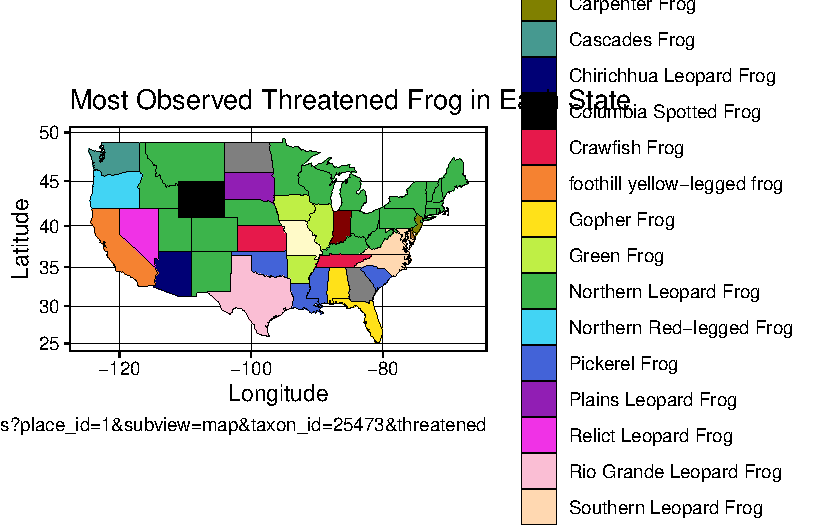
\includegraphics{MiniProject1_files/figure-pdf/unnamed-chunk-5-1.pdf}

\subsection{Joining for Interactive
Polygons}\label{joining-for-interactive-polygons}

\begin{Shaded}
\begin{Highlighting}[]
\NormalTok{states }\OtherTok{\textless{}{-}}\NormalTok{ states }\SpecialCharTok{|\textgreater{}}
  \FunctionTok{filter}\NormalTok{(}\SpecialCharTok{!}\NormalTok{(name }\SpecialCharTok{\%in\%} \FunctionTok{c}\NormalTok{(}\StringTok{"Alaska"}\NormalTok{, }\StringTok{"Hawaii"}\NormalTok{, }\StringTok{"Puerto Rico"}\NormalTok{))) }\SpecialCharTok{|\textgreater{}}
  \FunctionTok{select}\NormalTok{(}\StringTok{"name"}\NormalTok{, }\StringTok{"geometry"}\NormalTok{)}

\NormalTok{frogs\_interactive }\OtherTok{\textless{}{-}}\NormalTok{ frogs }\SpecialCharTok{|\textgreater{}}
  \FunctionTok{right\_join}\NormalTok{(states, }\AttributeTok{by =} \FunctionTok{c}\NormalTok{(}\StringTok{"state"} \OtherTok{=} \StringTok{"name"}\NormalTok{))}
\end{Highlighting}
\end{Shaded}

\begin{Shaded}
\begin{Highlighting}[]
\NormalTok{forest\_interactive }\OtherTok{\textless{}{-}}\NormalTok{ forests }\SpecialCharTok{|\textgreater{}}
  \FunctionTok{right\_join}\NormalTok{(states, }\AttributeTok{by =} \FunctionTok{c}\NormalTok{(}\StringTok{"state"} \OtherTok{=} \StringTok{"name"}\NormalTok{))}
\end{Highlighting}
\end{Shaded}

\subsection{Interactive Maps}\label{interactive-maps}

\begin{Shaded}
\begin{Highlighting}[]
\NormalTok{forest\_sf }\OtherTok{\textless{}{-}} \FunctionTok{st\_as\_sf}\NormalTok{(forest\_interactive) }\SpecialCharTok{|\textgreater{}}
  \FunctionTok{mutate}\NormalTok{(}\AttributeTok{forest\_cover =} \FunctionTok{trunc}\NormalTok{(forest\_cover))}

\NormalTok{pal }\OtherTok{\textless{}{-}} \FunctionTok{colorNumeric}\NormalTok{(}\StringTok{"Greens"}\NormalTok{, }\AttributeTok{domain =}\NormalTok{ forest\_sf}\SpecialCharTok{$}\NormalTok{forest\_cover)}

\NormalTok{forest\_sf }\OtherTok{\textless{}{-}}\NormalTok{ forest\_sf }\SpecialCharTok{|\textgreater{}}
  \FunctionTok{mutate}\NormalTok{(}\AttributeTok{labels =} \FunctionTok{str\_c}\NormalTok{(state, }\StringTok{": "}\NormalTok{, forest\_cover, }\StringTok{"\% forest cover"}\NormalTok{))}

\NormalTok{labels }\OtherTok{\textless{}{-}} \FunctionTok{lapply}\NormalTok{(forest\_sf}\SpecialCharTok{$}\NormalTok{labels, HTML)}
\FunctionTok{leaflet}\NormalTok{(forest\_sf) }\SpecialCharTok{|\textgreater{}}
  \FunctionTok{setView}\NormalTok{(}\SpecialCharTok{{-}}\DecValTok{96}\NormalTok{, }\FloatTok{37.8}\NormalTok{, }\DecValTok{4}\NormalTok{) }\SpecialCharTok{|\textgreater{}}
  \FunctionTok{addProviderTiles}\NormalTok{(}\StringTok{"Esri.WorldTopoMap"}\NormalTok{) }\SpecialCharTok{|\textgreater{}}
  \FunctionTok{addPolygons}\NormalTok{(}
    \AttributeTok{fillColor =} \SpecialCharTok{\textasciitilde{}}\FunctionTok{pal}\NormalTok{(forest\_cover),}
    \AttributeTok{weight =} \DecValTok{2}\NormalTok{,}
    \AttributeTok{opacity =} \DecValTok{1}\NormalTok{,}
    \AttributeTok{color =} \StringTok{"black"}\NormalTok{,}
    \AttributeTok{fillOpacity =} \FloatTok{0.6}\NormalTok{,}
    \AttributeTok{highlightOptions =} \FunctionTok{highlightOptions}\NormalTok{(}
      \AttributeTok{weight =} \DecValTok{5}\NormalTok{,}
      \AttributeTok{color =} \StringTok{"pink"}\NormalTok{,}
      \AttributeTok{fillOpacity =} \FloatTok{0.7}\NormalTok{,}
      \AttributeTok{bringToFront =} \ConstantTok{TRUE}\NormalTok{),}
    \AttributeTok{label =}\NormalTok{ labels,}
    \AttributeTok{labelOptions =} \FunctionTok{labelOptions}\NormalTok{(}
      \AttributeTok{style =} \FunctionTok{list}\NormalTok{(}\StringTok{"font{-}weight"} \OtherTok{=} \StringTok{"normal"}\NormalTok{, }\AttributeTok{padding =} \StringTok{"3px 8px"}\NormalTok{),}
      \AttributeTok{textsize =} \StringTok{"12px"}\NormalTok{,}
      \AttributeTok{direction =} \StringTok{"auto"}\NormalTok{)) }\SpecialCharTok{|\textgreater{}}
  \FunctionTok{addLegend}\NormalTok{(}\AttributeTok{pal =}\NormalTok{ pal, }\AttributeTok{title =} \StringTok{"\% Forest Coverage"}\NormalTok{, }\AttributeTok{values =} \SpecialCharTok{\textasciitilde{}}\NormalTok{forest\_cover, }\AttributeTok{opacity =} \FloatTok{0.7}\NormalTok{, }\AttributeTok{position =} \StringTok{"bottomright"}\NormalTok{) }\SpecialCharTok{|\textgreater{}}
  \FunctionTok{addScaleBar}\NormalTok{(}\AttributeTok{position =} \StringTok{"bottomleft"}\NormalTok{) }\SpecialCharTok{|\textgreater{}}
  \FunctionTok{addPopups}\NormalTok{(}\SpecialCharTok{{-}}\DecValTok{95}\NormalTok{, }\DecValTok{50}\NormalTok{, }\StringTok{"Percentage of Forest Cover in Each State"}\NormalTok{,}
              \AttributeTok{options =} \FunctionTok{popupOptions}\NormalTok{(}\AttributeTok{closeOnClick =} \ConstantTok{FALSE}\NormalTok{))}
\end{Highlighting}
\end{Shaded}

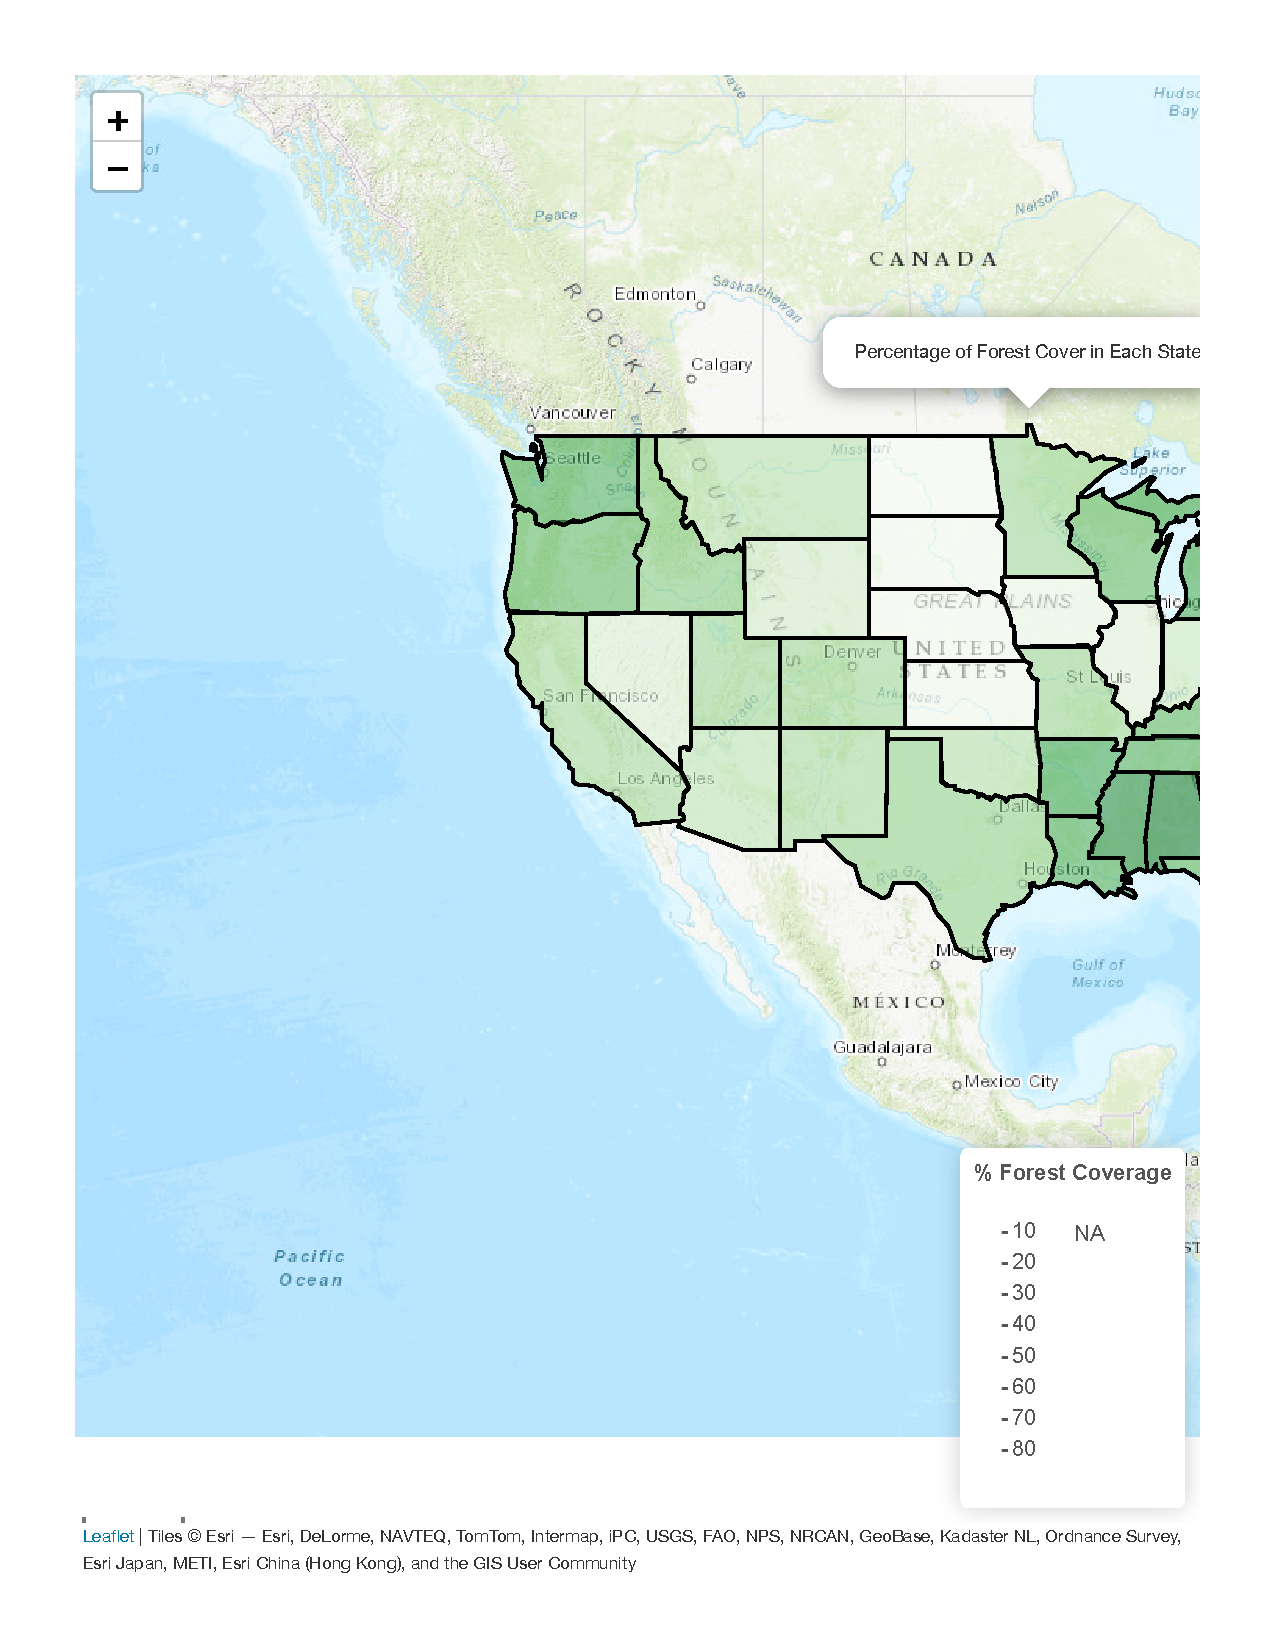
\includegraphics{MiniProject1_files/figure-pdf/unnamed-chunk-8-1.pdf}

\begin{Shaded}
\begin{Highlighting}[]
\NormalTok{frog\_sf }\OtherTok{\textless{}{-}} \FunctionTok{st\_as\_sf}\NormalTok{(frogs\_interactive) }
\NormalTok{pal }\OtherTok{\textless{}{-}} \FunctionTok{colorFactor}\NormalTok{(}\FunctionTok{c}\NormalTok{(}\StringTok{"\#800000"}\NormalTok{, }
                               \StringTok{"\#9A6324"}\NormalTok{, }
                               \StringTok{"\#808000"}\NormalTok{, }
                               \StringTok{"\#469990"}\NormalTok{, }
                               \StringTok{"\#000075"}\NormalTok{, }
                               \StringTok{"\#000000"}\NormalTok{, }
                               \StringTok{"\#e6194B"}\NormalTok{, }
                               \StringTok{"\#f58231"}\NormalTok{, }
                               \StringTok{"\#ffe119"}\NormalTok{, }
                               \StringTok{"\#bfef45"}\NormalTok{, }
                               \StringTok{"\#3cb44b"}\NormalTok{, }
                               \StringTok{"\#42d4f4"}\NormalTok{, }
                               \StringTok{"\#4363d8"}\NormalTok{,}
                               \StringTok{"\#911eb4"}\NormalTok{, }
                               \StringTok{"\#f032e6"}\NormalTok{, }
                               \StringTok{"\#fabed4"}\NormalTok{, }
                               \StringTok{"\#ffd8b1"}\NormalTok{,}
                               \StringTok{"\#fffac8"}\NormalTok{,}
                               \StringTok{"\#aaffc3"}\NormalTok{), }\AttributeTok{domain =}\NormalTok{ frog\_sf}\SpecialCharTok{$}\NormalTok{frog)}

\NormalTok{frog\_sf }\OtherTok{\textless{}{-}}\NormalTok{ frog\_sf }\SpecialCharTok{|\textgreater{}}
  \FunctionTok{mutate}\NormalTok{(}\AttributeTok{labels =} \FunctionTok{str\_c}\NormalTok{(}\StringTok{"The "}\NormalTok{, frog, }\StringTok{" is the most observed threatened frog in "}\NormalTok{, state))}

\NormalTok{labels }\OtherTok{\textless{}{-}} \FunctionTok{lapply}\NormalTok{(frog\_sf}\SpecialCharTok{$}\NormalTok{labels, HTML)}

\FunctionTok{leaflet}\NormalTok{(frog\_sf) }\SpecialCharTok{|\textgreater{}}
  \FunctionTok{setView}\NormalTok{(}\SpecialCharTok{{-}}\DecValTok{96}\NormalTok{, }\FloatTok{37.8}\NormalTok{, }\DecValTok{4}\NormalTok{) }\SpecialCharTok{|\textgreater{}}
  \FunctionTok{addProviderTiles}\NormalTok{(}\StringTok{"Esri.WorldTopoMap"}\NormalTok{) }\SpecialCharTok{|\textgreater{}}
  \FunctionTok{addPolygons}\NormalTok{(}
    \AttributeTok{fillColor =} \SpecialCharTok{\textasciitilde{}}\FunctionTok{pal}\NormalTok{(frog),}
    \AttributeTok{weight =} \DecValTok{2}\NormalTok{,}
    \AttributeTok{opacity =} \DecValTok{1}\NormalTok{,}
    \AttributeTok{color =} \StringTok{"black"}\NormalTok{,}
    \AttributeTok{fillOpacity =} \FloatTok{0.7}\NormalTok{,}
    \AttributeTok{highlightOptions =} \FunctionTok{highlightOptions}\NormalTok{(}
      \AttributeTok{weight =} \DecValTok{5}\NormalTok{,}
      \AttributeTok{color =} \StringTok{"pink"}\NormalTok{,}
      \AttributeTok{fillOpacity =} \FloatTok{0.7}\NormalTok{,}
      \AttributeTok{bringToFront =} \ConstantTok{TRUE}\NormalTok{),}
    \AttributeTok{label =}\NormalTok{ labels,}
    \AttributeTok{labelOptions =} \FunctionTok{labelOptions}\NormalTok{(}
      \AttributeTok{style =} \FunctionTok{list}\NormalTok{(}\StringTok{"font{-}weight"} \OtherTok{=} \StringTok{"normal"}\NormalTok{, }\AttributeTok{padding =} \StringTok{"3px 8px"}\NormalTok{),}
      \AttributeTok{textsize =} \StringTok{"12px"}\NormalTok{,}
      \AttributeTok{direction =} \StringTok{"auto"}\NormalTok{)) }\SpecialCharTok{|\textgreater{}}
  \FunctionTok{addLegend}\NormalTok{(}\AttributeTok{pal =}\NormalTok{ pal, }\AttributeTok{title =} \StringTok{"Frogs Observed"}\NormalTok{, }\AttributeTok{values =} \SpecialCharTok{\textasciitilde{}}\NormalTok{frog, }\AttributeTok{opacity =} \FloatTok{0.7}\NormalTok{, }\AttributeTok{position =} \StringTok{"bottomright"}\NormalTok{) }\SpecialCharTok{|\textgreater{}}
  \FunctionTok{addScaleBar}\NormalTok{(}\AttributeTok{position =} \StringTok{"bottomleft"}\NormalTok{)}
\end{Highlighting}
\end{Shaded}

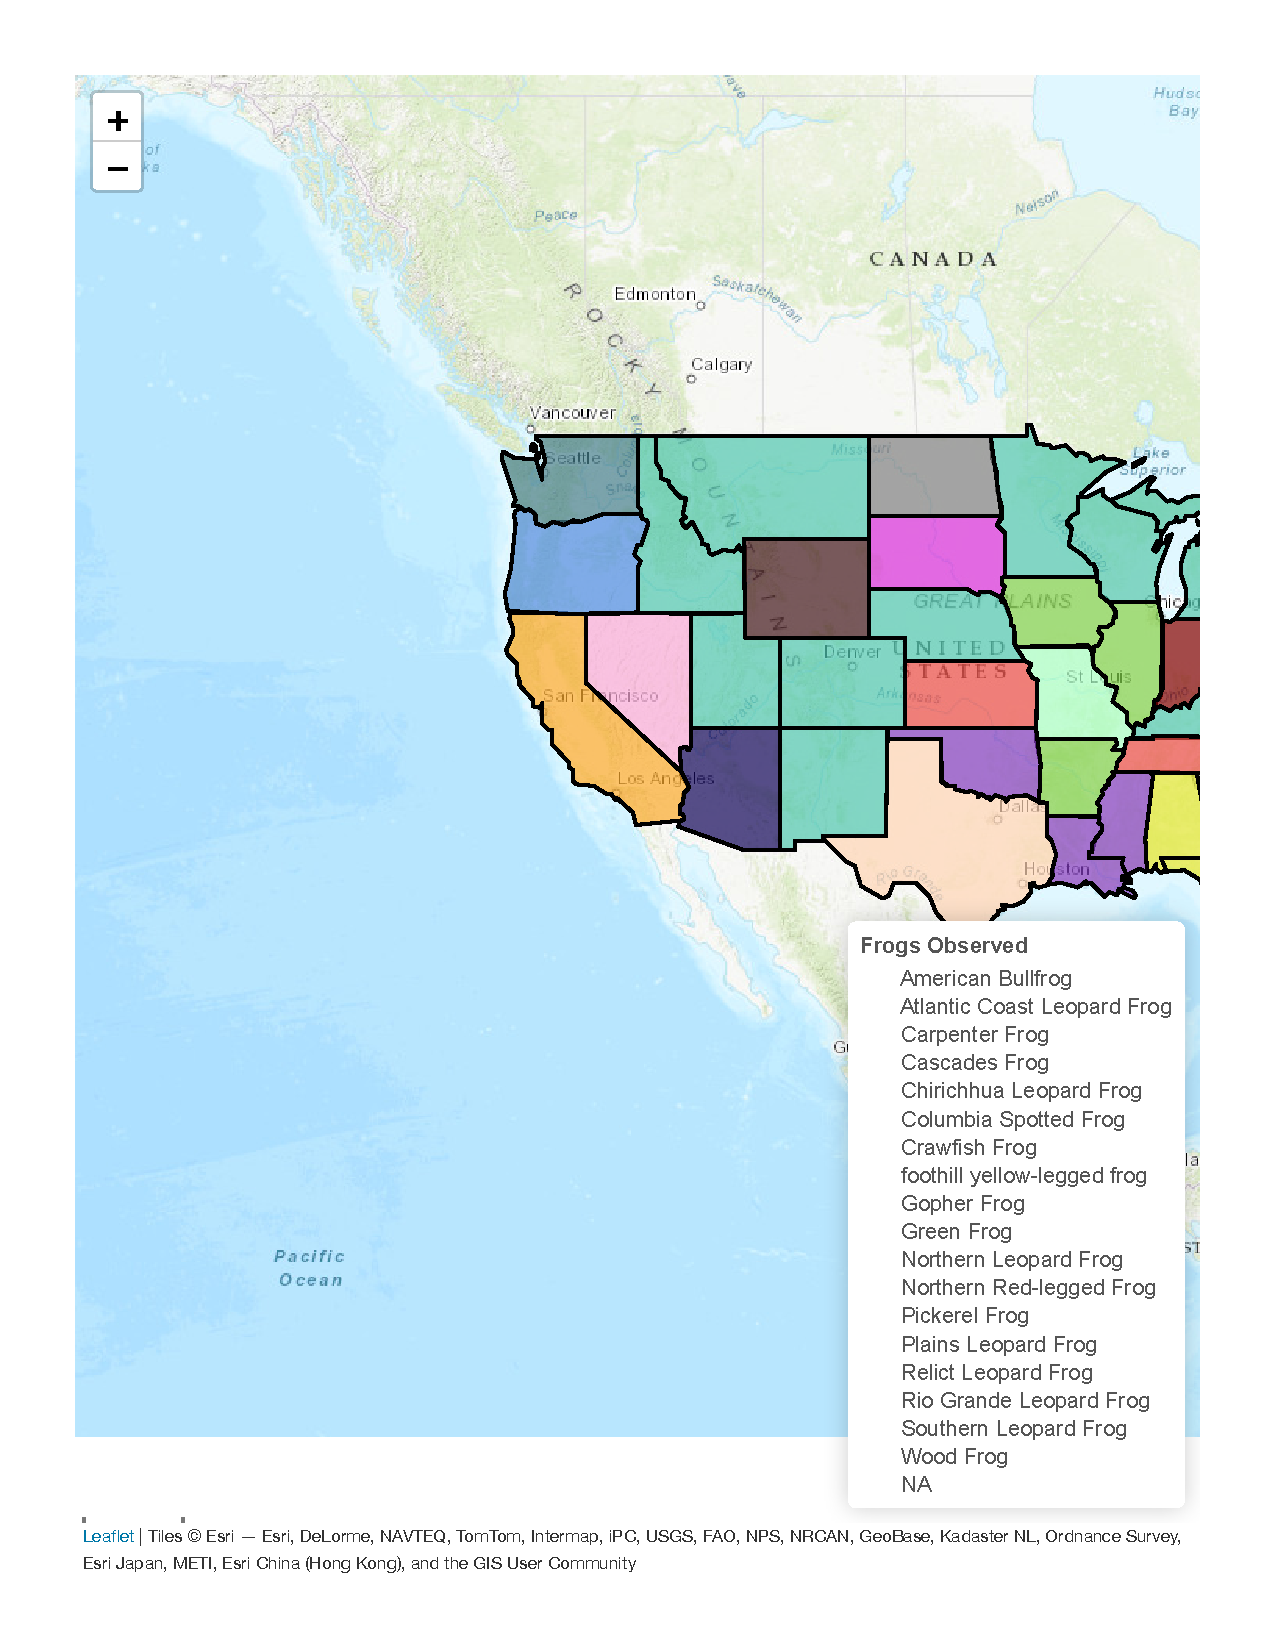
\includegraphics{MiniProject1_files/figure-pdf/unnamed-chunk-9-1.pdf}




\end{document}
